\section{Phase 1, Architecture A0: Dense Flash
LegalGPT}\label{phase-1-architecture-a0-dense-flash-legalgpt}

\textbf{Reproducible implementation, modeling decisions, training
procedure and evaluation protocol}

\emph{This is the A0 contribution to the capstone final report. It is
intended to be inserted into the supplied course LaTeX report template,
alongside results and contributions from other phases. Implementation
details below are verified against the supplied A0 Python source; absent
results are not manufactured.}

\subsection{1. Task formulation and architecture
overview}\label{task-formulation-and-architecture-overview}

Architecture A0 is a \textbf{from-scratch, decoder-only autoregressive
Transformer} for continuation of legal text. The official task presents
a 512-\textbf{word} prompt and requests a 128-\textbf{word}
continuation. Word counts are based on whitespace separation; a 512-word
sequence generally maps to an unequal number of Byte-Level BPE tokens.
During pretraining, instead of learning on 512→128 word pairs, A0
predicts every next BPE token in a fixed-length 2,048-token sequence
sampled from a packed legal-text corpus. The model contains \textbf{12
decoder blocks, 768 hidden features, 12 attention heads of 64 dimensions
each, a 2,048-dimensional SwiGLU intermediate transformation,
Pre-RMSNorm, RoPE, causal self-attention, and tied output/input
embeddings}. The nominal number of unique parameters at vocabulary size
32,768 is \textbf{110,119,680}.

\begin{figure}
\centering
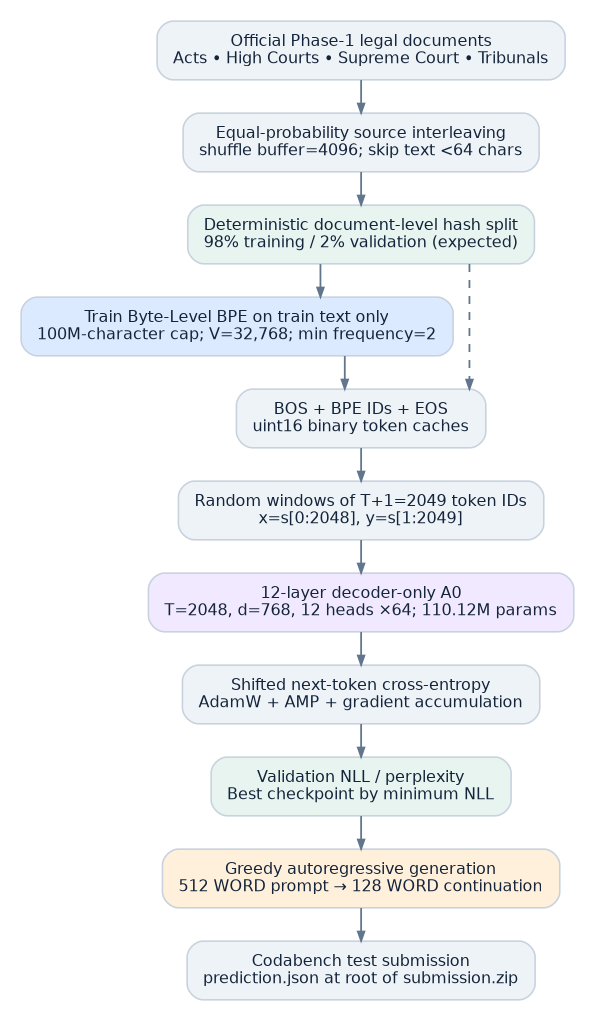
\includegraphics{../figures/01_end_to_end.png}
\caption{Full pipeline}
\end{figure}

The design objective is to develop a domain-trained baseline within the
capstone's stipulated parameter range, while providing straightforward
autoregressive pretraining and efficient cached generation.
Justifications described below are design rationale, not empirically
validated superiority claims absent controlled comparisons.

\subsection{2. Dataset loading, train/validation isolation and corpus
representation}\label{dataset-loading-trainvalidation-isolation-and-corpus-representation}

The implementation streams four official source files from Hugging Face
dataset \texttt{Exploration-Lab/CS-781-Capstone}:
\texttt{train\_acts.json}, \texttt{train\_high\_courts.json},
\texttt{train\_supreme\_court.json}, and \texttt{train\_tribunals.json}
under \texttt{Phase\_1\_Pretraining/Train/}. The default
\texttt{mix\_mode="equal"} creates shuffled streams (buffer size 4,096)
and picks an available source uniformly for each document yielded. Its
equal weighting is a \textbf{selection policy, not a guarantee of equal
token mass}, because source documents have different lengths. A combined
\texttt{phase\_1} dataset streaming fallback is implemented if
source-level streaming fails. Text extraction uses multiple supported
field names, recursively handles simple wrappers and rejects texts
shorter than 64 characters.

Train and validation are separated deterministically at \textbf{document
level} rather than on randomly sampled token windows. A key constructed
from source, record identity and SHA1 of a text prefix is hashed again;
keys whose normalized eight-byte SHA1 value is below 0.02 enter
validation. The expected validation fraction is 2\% of such keys.
Validation documents are excluded both when fitting the tokenizer and
when building the language-model training token cache. The code does not
implement near-duplicate matching between distinct records; therefore
this is a deterministic partition, not proof of semantic deduplication.

The program sets default caps of \textbf{200,000,000 training BPE IDs}
and \textbf{5,000,000 validation BPE IDs}. Document IDs are encoded and
appended without padding as
\texttt{{[}BOS,\ ...document\ token\ IDs...,\ EOS{]}} to separate
\texttt{uint16} binary streams. A document can be truncated to respect
the cache cap, and continuous training windows can straddle EOS/BOS
boundaries. There is no reset-of-attention at document boundaries, and
EOS remains an ordinary training target. These are material algorithmic
details rather than incidental implementation choices.

\subsection{3. Tokenizer training: the complete Byte-Level BPE
protocol}\label{tokenizer-training-the-complete-byte-level-bpe-protocol}

A0 imports the Rust-backed Hugging Face \texttt{tokenizers}
implementation and trains a \textbf{new Byte-Level BPE model} on
official legal text. The algorithm itself is not written from scratch
and no pretrained vocabulary is loaded. The configuration is
\texttt{Tokenizer(BPE(unk\_token="\textless{}unk\textgreater{}"))} with
\texttt{ByteLevel(add\_prefix\_space=False)},
\texttt{ByteLevelDecoder()}, and
\texttt{BpeTrainer(vocab\_size=32768,min\_frequency=2,special\_tokens={[}"\textless{}pad\textgreater{}","\textless{}bos\textgreater{}","\textless{}eos\textgreater{}","\textless{}unk\textgreater{}"{]},show\_progress=True)}.
The raw text iterator supplies non-validation documents until the first
\textbf{100 million Python string characters} have been processed, with
the final supplied text optionally truncated to the remaining quota. No
extra normalizer or tokenizer post-processor is specified.

Byte-Level BPE starts from byte-level units and learns a succession of
merges. At each iteration, the trainer counts \textbf{adjacent pairs
inside its pre-tokenized sequences}, picks the most frequent eligible
pair (minimum frequency 2), assigns a merged symbol and updates the
segmentation; later merge priorities depend on earlier merges. It
terminates at the requested vocabulary size or when remaining eligible
merges are exhausted. The program does not set a separate merge count
\(M\) or a top-k pair list. The final actual vocabulary size and
metadata are saved in \texttt{tokenizer/tokenizer\_meta.json}, and
learned symbol IDs/merge rules in \texttt{tokenizer/tokenizer.json}. The
exact realized merge list, IDs and final size require this generated
tokenizer file; they cannot be inferred from configuration alone. The
tokenizer is thereafter fixed: it maps text deterministically to subword
IDs, while the Transformer learns the trainable semantic embeddings of
those IDs.

Top-k sampling, nucleus sampling, beam search and temperature scaling
are \textbf{not BPE training algorithms}. They are choices for
generating the next token from a trained language model. In A0, the
selection of BPE merges is frequency-driven and greedy; inference
decoding is separately configured as described in Section 7.

\subsection{4. Transformer computation: every representation and
sublayer}\label{transformer-computation-every-representation-and-sublayer}

For one training example of length \(T=2048\), the input token IDs have
shape \([T]\). An embedding matrix \(E\in\mathbb R^{32768\times768}\)
maps these indices to \(H^{(0)}\in\mathbb R^{2048\times768}\). The full
default micro-batch has shape \([1,2048,768]\), but the following
ignores the batch dimension. A0 does not add a learned absolute position
vector to these embeddings; the attention projections use RoPE for
position.

\begin{figure}
\centering
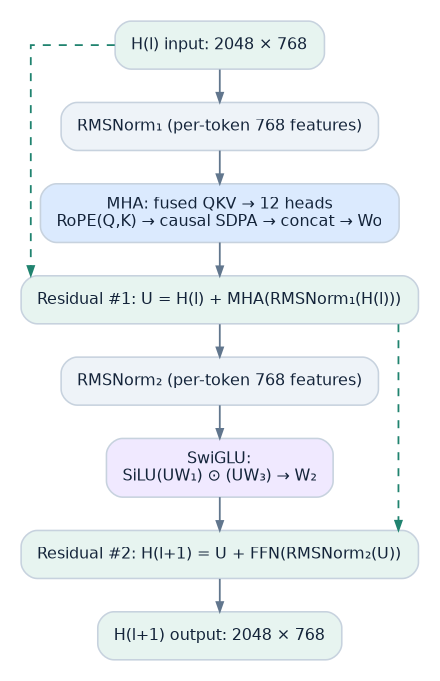
\includegraphics{../figures/02_block.png}
\caption{Decoder block}
\end{figure}

In block \(\ell\), the first step is
\(\widetilde H=\mathrm{RMSNorm}_1(H^{(\ell)})\), independently
normalizing each token's \textbf{768 features} (not features across
token positions):

\[
\mathrm{RMSNorm}(x)_j = \gamma_j x_j\big/\sqrt{\frac1{768}\sum_{k=1}^{768}x_k^2+10^{-6}}.
\]

RMSNorm uses an initialized-to-one learned gain vector, no centering and
no learned bias. The code evaluates its mean squares in float32 before
casting back for AMP. Next, a fused bias-free
\texttt{nn.Linear(768,2304)} produces Q, K, V, each \([2048,768]\), and
reshapes them into 12 heads, each having Q/K/V of shape \([2048,64]\).
Every head observes all 2,048 positions; the 768 \textbf{feature}
channels are divided among heads, not the tokens.

\begin{figure}
\centering
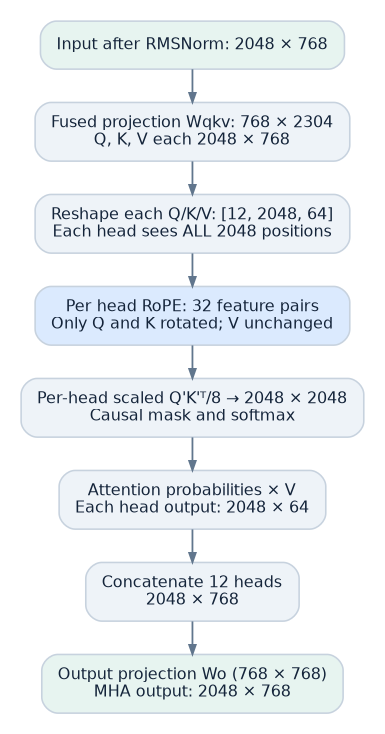
\includegraphics{../figures/03_heads.png}
\caption{Per-head attention}
\end{figure}

Rotary Position Embedding groups each 64-dimensional Q and K vector into
32 adjacent pairs. For token position \(m=0,\ldots,2047\) and coordinate
pair \(i=0,\ldots,31\), the frequency and angle are

\[
\theta_i=10000^{-2i/64},\qquad \phi_{m,i}=m\theta_i.
\]

Each pair \((a,b)\) becomes
\((a\cos\phi-b\sin\phi,\;a\sin\phi+b\cos\phi)\). Q and K are rotated; V
is untouched. Equivalently, the position-dependent block-diagonal
\(64\times64\) rotation \(R_m\) yields \(q'_m=R_m q_m\) and
\(k'_m=R_m k_m\), and

\[
(R_mq)^\top(R_nk)=q^\top R_{n-m}k.
\]

Thus the query-key compatibility is explicitly sensitive to relative
token positions. Frequencies are fixed, and RoPE adds \textbf{zero
learned parameters}. The source precomputes sine/cosine buffers for up
to 2,048 positions and uses a cache-length offset during autoregressive
generation.

Attention per head computes \(S=Q'K'^\top/\sqrt{64}=Q'K'^\top/8\), a
\([2048,2048]\) score matrix conceptually. Its causal mask suppresses
future positions; softmax yields attention weights that multiply the
corresponding V matrix, producing \([2048,64]\) per head. The
implementation calls PyTorch's \texttt{scaled\_dot\_product\_attention}
(SDPA), enabling CUDA Flash, memory-efficient and math backends. An
optimized Flash kernel may be dispatched if supported; the package does
\textbf{not} demonstrate a profiler-confirmed kernel choice. Outputs
from 12 heads concatenate to \([2048,768]\) and pass through a bias-free
\(768\to768\) projection \(W_O\). The first residual operation is

\[
U=H^{(\ell)}+\operatorname{MHA}(\operatorname{RMSNorm}_1(H^{(\ell)})).
\]

A second RMSNorm operates on U. SwiGLU applies two \emph{independent},
fully connected \(768\to2048\) transformations, \(a=xW_1\) and
\(b=xW_3\), to \textbf{each token separately}. The gated intermediate is
\(z=\mathrm{SiLU}(a)\odot b\), where
\(\mathrm{SiLU}(a)=a\odot\sigma(a)\) contains a sigmoid. Branch b is an
\textbf{unbounded linear projection} rather than a bounded sigmoid gate;
multiplicative interaction controls sign/magnitude of hidden features.
The final \(2048\to768\) matrix \(W_2\) restores the residual width:

\[
\mathrm{SwiGLU}(x)=\big[\mathrm{SiLU}(xW_1)\odot(xW_3)\big]W_2,
\qquad H^{(\ell+1)}=U+\mathrm{SwiGLU}(\mathrm{RMSNorm}_2(U)).
\]

\begin{figure}
\centering
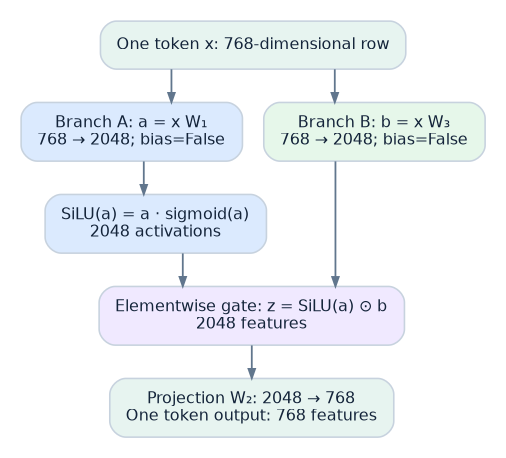
\includegraphics{../figures/04_swiglu.png}
\caption{SwiGLU branches}
\end{figure}

Each layer has two RMSNorms and two residual additions. Every one of 12
blocks has distinct learned weights, preserving the \([2048,768]\)
hidden shape across blocks. After the last block, the final RMSNorm
produces \(H_f\in\mathbb R^{2048\times768}\), and the vocabulary head
computes \(Z=H_fE^\top\in\mathbb R^{2048\times32768}\). Crucially, \(E\)
is the \textbf{same learned matrix} used to embed input IDs; the LM head
does not introduce an independent second 25.2M-parameter matrix. There
is no final softmax inside \texttt{LegalGPT.forward}; cross-entropy
consumes logits directly.

\textbf{Parameter derivation.} Embeddings plus tied head contribute
\(32768\cdot768=25,165,824\); each Transformer block contributes QKV
\(3d^2\), attention output \(d^2\), SwiGLU \(3dd_{ff}\) and two norm
gains \(2d\), totaling 7,079,424. Twelve blocks contribute 84,953,088,
with a final 768-element norm gain. Total
\(P=25,165,824+84,953,088+768=110,119,680\). Linear projections have
\texttt{bias=False}; therefore no additional bias counts are hidden.

\subsection{5. Training objective, initialization, numerical settings
and
optimizer}\label{training-objective-initialization-numerical-settings-and-optimizer}

\texttt{RandomMemmapBatcher} reads \textbf{2,049 consecutive IDs},
generates input \texttt{x=arr{[}:,:-1{]}} and shifted targets
\texttt{y=arr{[}:,1:{]}}, each of length 2,048. The training loss is
mean autoregressive cross-entropy:

\[
\mathcal L(\theta)=-\frac1{T}\sum_{t=0}^{T-1}\log p_\theta(s_{t+1}\mid s_0,\ldots,s_t),\quad T=2048.
\]

The sum includes any EOS/BOS labels inside the packed window. Since all
T input positions undergo causally masked attention, these T next-token
predictions can be processed in parallel; \textbf{the model does not
generate 2,048 tokens sequentially in the training loop}.

All embedding and linear weights initialize as Normal(mean 0, standard
deviation 0.02). Attention-output and SwiGLU-output projection weights
are subsequently scaled to standard deviation \(0.02/\sqrt{2L}\) with
\(L=12\); RMSNorm gains initialize to one. No pretrained Transformer
weights are loaded. A0 uses AdamW with peak learning rate
\(3\times10^{-4}\), betas (0.9, 0.95), epsilon \(10^{-8}\), weight decay
0.1 for tensors with at least two dimensions and zero decay for 1-D
parameters, a \textbf{2\% linear warmup}, and cosine decay to
\textbf{10\%} of peak LR. Global gradient-norm clipping threshold is
1.0.

The default micro-batch size is one 2,048-token sequence, accumulated
for 32 micro-batches before an optimizer step, giving \textbf{65,536
processed token positions/step} on one GPU. The code's target of 200M
processed positions implies \(\lceil200,000,000/65,536\rceil=3052\)
planned updates, not proof of completed steps. It uses activation
checkpointing per block, CUDA autocast BF16 if supported or FP16 with
GradScaler, and can use NCCL distributed data parallelism. The code
enables optimized SDPA backends but the precise backend remains
hardware-dependent.

\begin{figure}
\centering
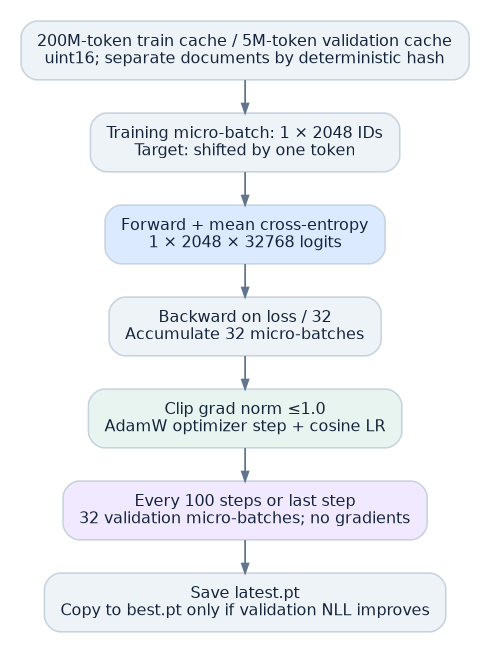
\includegraphics{../figures/05_train_validate.png}
\caption{Training and validation}
\end{figure}

\subsection{6. Validation, model selection and checkpoint
integrity}\label{validation-model-selection-and-checkpoint-integrity}

The main validation criterion is \textbf{held-out next-token
cross-entropy}, computed with \texttt{no\_grad()} over 32 randomly
sampled validation micro-batches every 100 optimizer updates and at
training end. Perplexity is reported as \(\exp(\mathrm{NLL})\). At each
such evaluation the script atomically saves \texttt{latest.pt}
(including model weights, optimizer state, scaler state, step, best NLL,
processed-token count and saved configs) and copies it to
\texttt{best.pt} if the NLL \textbf{strictly improves}. Training resumes
from \texttt{latest.pt}, whereas evaluation/inference loads
\texttt{best.pt} if present, otherwise latest. Resumption does not save
and restore every RNG state, so exact bitwise equivalence to
uninterrupted training is not guaranteed. No actual \texttt{best.pt} or
training metrics were present in the supplied source files; this
document therefore makes \textbf{no claim about achieved loss,
perplexity or convergence}.

A distinct \textbf{generation validation} is constructed from held-out
documents with at least 640 whitespace words, selecting one reproducible
640-word window per document, splitting it into 512-word prompt and
128-word reference, and storing up to 128 such examples. The default
local evaluation runs 32 examples and reports stemmed ROUGE-L F1 and
SacreBLEU-4 normalized to {[}0,1{]}. Local BERTScore is deliberately
disabled by default because the scorer involves external pretrained
weights. Codabench is the authoritative source for the task's primary
BERTScore F1. Training and scoring protocols are not interchangeable: no
gradients flow through BERTScore during A0 training.

\subsection{7. Exact generation algorithm and token-to-word stopping
rule}\label{exact-generation-algorithm-and-token-to-word-stopping-rule}

For inference, A0 loads a saved checkpoint and tokenizer, and encodes a
512-word input prompt into a \textbf{variable number} of BPE tokens
\(N-1\), prepending BOS so there are \(N\) ID positions. It rejects
\(N\ge2032\) and does not dynamically crop prompts. Prefill passes the
entire \([1,N]\) sequence through the 12-layer model, returning logits
\([1,N,V]\) and per-block KV caches; only the \textbf{last-position}
vocabulary logits \([1,V]\) are used to predict the next token.
Thereafter the generator runs the model on \textbf{one new token per
step}, reusing cached K/V with the appropriate RoPE positional offset.
The number of attention heads and all weight dimensions remain fixed
even though N changes at inference.

\begin{figure}
\centering
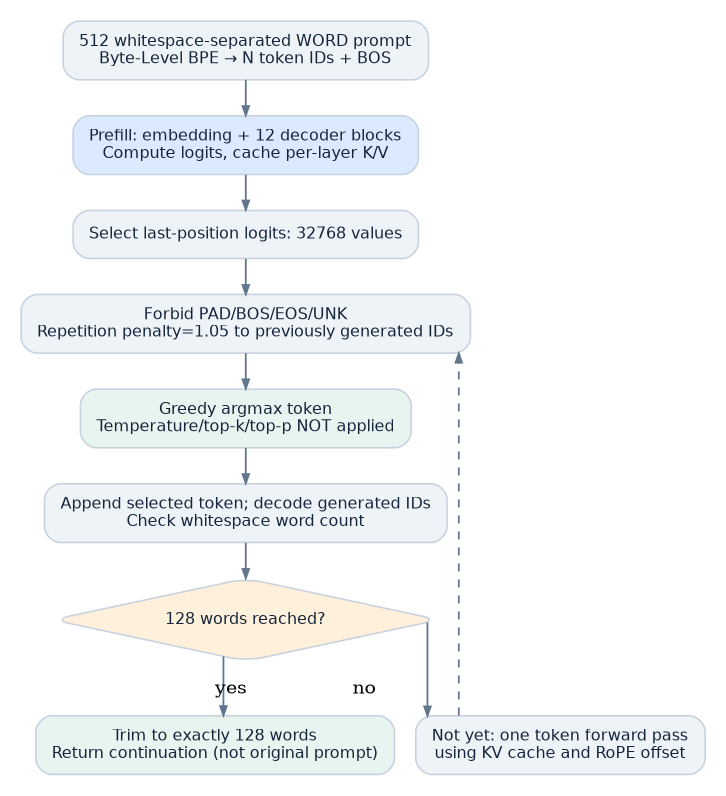
\includegraphics{../figures/06_generation.png}
\caption{Autoregressive continuation}
\end{figure}

The \textbf{default} strategy is \textbf{greedy decoding}: first forbid
PAD, BOS, EOS and UNK; apply sign-aware repetition penalty 1.05 only to
\emph{previously generated} token IDs; then return the highest remaining
logit. Because greedy uses \texttt{argmax} directly, configured
\texttt{temperature=0.8}, \texttt{top\_k=50} and \texttt{top\_p=0.90} do
\textbf{not} affect the default. Optional \texttt{topk} and
\texttt{nucleus} modes use temperature-scaled probabilities and seeded
multinomial sampling; no beam search is coded. The generator repeatedly
decodes all accumulated generated BPE IDs and checks
\texttt{len(re.findall(r"\textbackslash{}S+",text))}. It stops and trims
when it reaches \textbf{128 words}, not 128 BPE IDs, with a hard limit
of \texttt{min(384,2048-N)} generated token IDs. If insufficient words
appear by this cap, the code raises an exception instead of silently
padding or producing a shorter answer. EOS is excluded to avoid early
termination in the fixed-word output task. Any final 128-word output is
text only, without the original input prompt.

The Codabench output format is exactly a ZIP with
\texttt{prediction.json} at its root, mapping each official test ID to a
JSON object containing only \texttt{text}, whose value contains exactly
128 whitespace-separated words. This is \textbf{separate} from the
capstone's final report/code ZIP, for which the 7 November 2026 staff
announcement requires \texttt{code/} and \texttt{report/} at the root of
a single archive and a public GitHub link in the report. The present
artifact documents A0 only, not the best architecture across all phases.

\subsection{8. Computation and memory
implications}\label{computation-and-memory-implications}

With \(P=110,119,680\) learned scalars, float32 parameter storage is
about \textbf{420 MiB}; gradients require approximately another
\textbf{420 MiB} when allocated, and two Adam moments approximately
\textbf{840 MiB}, before activations or device allocator overhead. A
training logits tensor of shape \([1,2048,32768]\) has
\textbf{67,108,864 elements}, requiring \textasciitilde128 MiB in
FP16/BF16 or 256 MiB in float32. Naively materializing all head scores
would involve \(12\times2048\times2048\) entries per layer
(\textasciitilde96 MiB in FP16), while a suitable fused Flash SDPA
kernel may avoid writing that full score tensor to global memory. One
fully populated 12-layer BF16/FP16 K/V cache at T=2048 requires
\textasciitilde72 MiB. These are \textbf{analytical tensor estimates};
the actual peak GPU allocation and selected attention kernel were not
measured in the supplied artifacts. The 200M-token \texttt{uint16}
training cache occupies \textasciitilde381.5 MiB on disk at the
configured cap.

\subsection{9. Methodological rationale, limitations and reproducibility
status}\label{methodological-rationale-limitations-and-reproducibility-status}

\textbf{Rationales.} Byte-Level BPE trained on the domain can learn
frequent legal terminology and preserves byte-level coverage. A
decoder-only causal objective matches continuation generation. MHA
provides parallel learned token-interaction subspaces; RoPE encodes
relative offsets without learned positional weights; Pre-RMSNorm
improves scaling of sublayer inputs and residual pathways; SwiGLU
provides multiplicative feature interactions; embedding tying reduces
parameter count and aligns output token scoring with learned input
embeddings; AMP, activation checkpointing and SDPA address computational
cost; AdamW and cosine decay are standard stable baseline choices.
Greedy inference offers a deterministic generation baseline. These are
\textbf{engineering motivations}, not evidence that this configuration
outperforms alternatives.

\textbf{Limitations explicitly visible in source.} The packed-corpus
objective attends across BOS/EOS boundaries; there is no sequence
masking at document ends. Training data are streamed without explicit
near-duplicate removal. The source's dataset URLs resolve mutable
\texttt{main} versions; dependency versions are bounded below but not
pinned. Tokenizer/cache artifacts are reused based on existence rather
than verified config compatibility. Resumed runs omit RNG-state
restoration. A prompt consuming too much of the 2,048 BPE context raises
an error; 384 generated BPE tokens may not always yield 128 words. The
selected CUDA attention backend is not profiler-confirmed. No training
or evaluation output is included in this original A0 source package.

\textbf{Reproduction status.} The supplied original Python file
successfully passes its built-in tiny-model forward/cache self-test. No
full-corpus tokenizer fit, 110M-parameter training, best checkpoint
validation or Codabench scoring was run to create this document. This
prevents scientifically unsupported numerical result claims. Exact
commands, tensor ledger, entire source code, complete options,
environment/data caveats and validation checklist are in the
accompanying \texttt{README.md},
\texttt{docs/A0\_TECHNICAL\_REFERENCE.md} and
\texttt{docs/CODE\_MAP.md}.

\subsection{10. A0-specific AI assistance
disclosure}\label{a0-specific-ai-assistance-disclosure}

AI assistance was used in auditing and explaining the provided A0 source
implementation, deriving explicit tensor shapes and parameter/memory
estimates, drafting the methodological documentation, and generating
illustrative diagrams. The source implementation, executed experimental
results, and final academic claims must be verified separately. No
experimental metric or completed training run has been invented for the
report.

\emph{References:} Original \texttt{architecture\_a\_legalgpt.py}
supplied by the student; CS781 Modules 2.2 and 2.3 lecture PDFs supplied
in this conversation; Hugging Face \texttt{tokenizers} and PyTorch API
conventions used by the code; RoFormer, arXiv:2104.09864; final
report-code submission announcement (7 November 2026).
